%!TEX program = pdflatex
\documentclass[11pt,en]{elegantpaper}

\title{Template for the Survey Paper}
\author{Anonymous}
\institute{Anonymous}

% cmd for this doc
\usepackage{array}
\newcommand{\ccr}[1]{\makecell{{\color{#1}\rule{1cm}{1cm}}}}

\begin{document}

\maketitle

\begin{abstract}
This article is an explanatory document for the template of a review paper on scientific research methods and practical courses. This template is based on the article class of LATEX. If you have any questions, please contact the course assistant\footnote[1]{wang\_xiaodong@stu.pku.edu.cn\\2401111937@stu.pku.edu.cn\\ yuxueqing@pku.edu.cn} or provide feedback in the course group.

\keywords{\LaTeX{}, Survey Paper, Template}
\end{abstract}


\section{Course Requirements}

The Scientific Research Methods and Practice course aims to cultivate students' independent research and academic writing abilities. Each student is required to complete a paper survey. The specific requirements are as follows.

\subsection{Content Requirements}
\begin{itemize}
    \item The paper needs to introduce at least 5 papers in relevant research fields.
    \item The paper should have a clear structure, including abstract, introduction, review, discussion, and conclusion.
    \item The paper should include a figure or table comparing the similarities and differences of existing work, accompanied by appropriate explanatory text.
    \item The word count range of the paper should be between 1500 and 2500 words, excluding references.
    \item The paper can be written in Chinese or English, but it is necessary to ensure accurate and clear language expression.
\end{itemize}

\subsection{Submission Deadline}
The paper needs to be submitted before \textbf{October 28th}. Late submissions will not be accepted. Please make sure to schedule the completion of the paper in advance and ensure timely submission.

\subsection{Submission Platform}
The paper should be submitted through the HotCRP platform. Please click on the following link to enter the submission page: \href{https://pku-cs25sci.hotcrp.com/}{https://pku-cs25sci.hotcrp.com}。
 
\subsection{Peer review rules}
Each paper will be reviewed by three classmates, and the review process will follow the following principles:

\textbf{Reviewer selection}: Three peer reviewers will be assigned to each paper. The selection of reviewers will remain anonymous.

\textbf{Review Criteria}: Reviewers are required to evaluate the paper based on the following criteria:
\begin{itemize}
    \item The structure and organization of the paper.
    \item The accuracy and comprehensiveness of the paper's synthesis of relevant literature.
    \item The accuracy and fluency of the language expression in the paper.
    \item The depth and breadth of the paper.
    \item The insight and value of the discussion and conclusion of the paper.
\end{itemize}

\textbf{Submit review comments}: Reviewers are required to submit review comments within the designated time frame, including ratings and suggestions for the paper. The evaluation opinions will have an impact on the final grade of the paper.

\textbf{Attention}: To provide a fair and transparent review process, students should complete their papers within the prescribed time and adhere to the principle of integrity, and should not plagiarize or plagiarize others' works. If you have any questions or need further guidance, please feel free to contact the course teacher or teaching assistant at any time.

\section{Template Usage Instructions}

This template is based on the standard \LaTeX{} article class, hence the arguments of article class are acceptable. The page setting of this template is \lstinline {a4paper}, and the font size of the main text is \lstinline {11pt}. Please do not modify it.

\begin{lstlisting}
\documentclass[a4paper,11pt]{elegantpaper}
\end{lstlisting}

\subsection{Use of Chinese and English templates}

\begin{itemize}
    \item For Chinese, please use \lstinline{template-cn.tex} as template, and use \hologo{XeLaTeX} for compile.
    \item For English, please use \lstinline{template-en.tex}as template, and use \hologo{pdfLaTeX} or \hologo{XeLaTeX} for compile.
\end{itemize}

Language mode option \lstinline{lang} allows two alternative inputs, \lstinline{lang=en} (default)  for English or \lstinline{lang=cn} for Chinese. \lstinline{lang=cn} will make the caption of figure/table, abstract name, refname etc. Chinese. You can use this option as
\begin{lstlisting}
\documentclass[lang=cn]{elegantpaper} % or
\documentclass{cn}{elegantpaper} 
\end{lstlisting}
\textbf{Note:} Under the English mode \lstinline{lang=en}, Chinese characters are not allowed. To type in Chinese, please load  \lstinline{ctex} or \lstinline{xeCJK} package at the preamble as:
\begin{lstlisting}
\usepackage[UTF8,scheme=plain]{ctex}
\end{lstlisting}

\subsection{Figures and Tables}

\subsubsection{Figures}
Here is a code example for inserting an image.
\begin{lstlisting}
\begin{figure}[!htb]
    \centering
    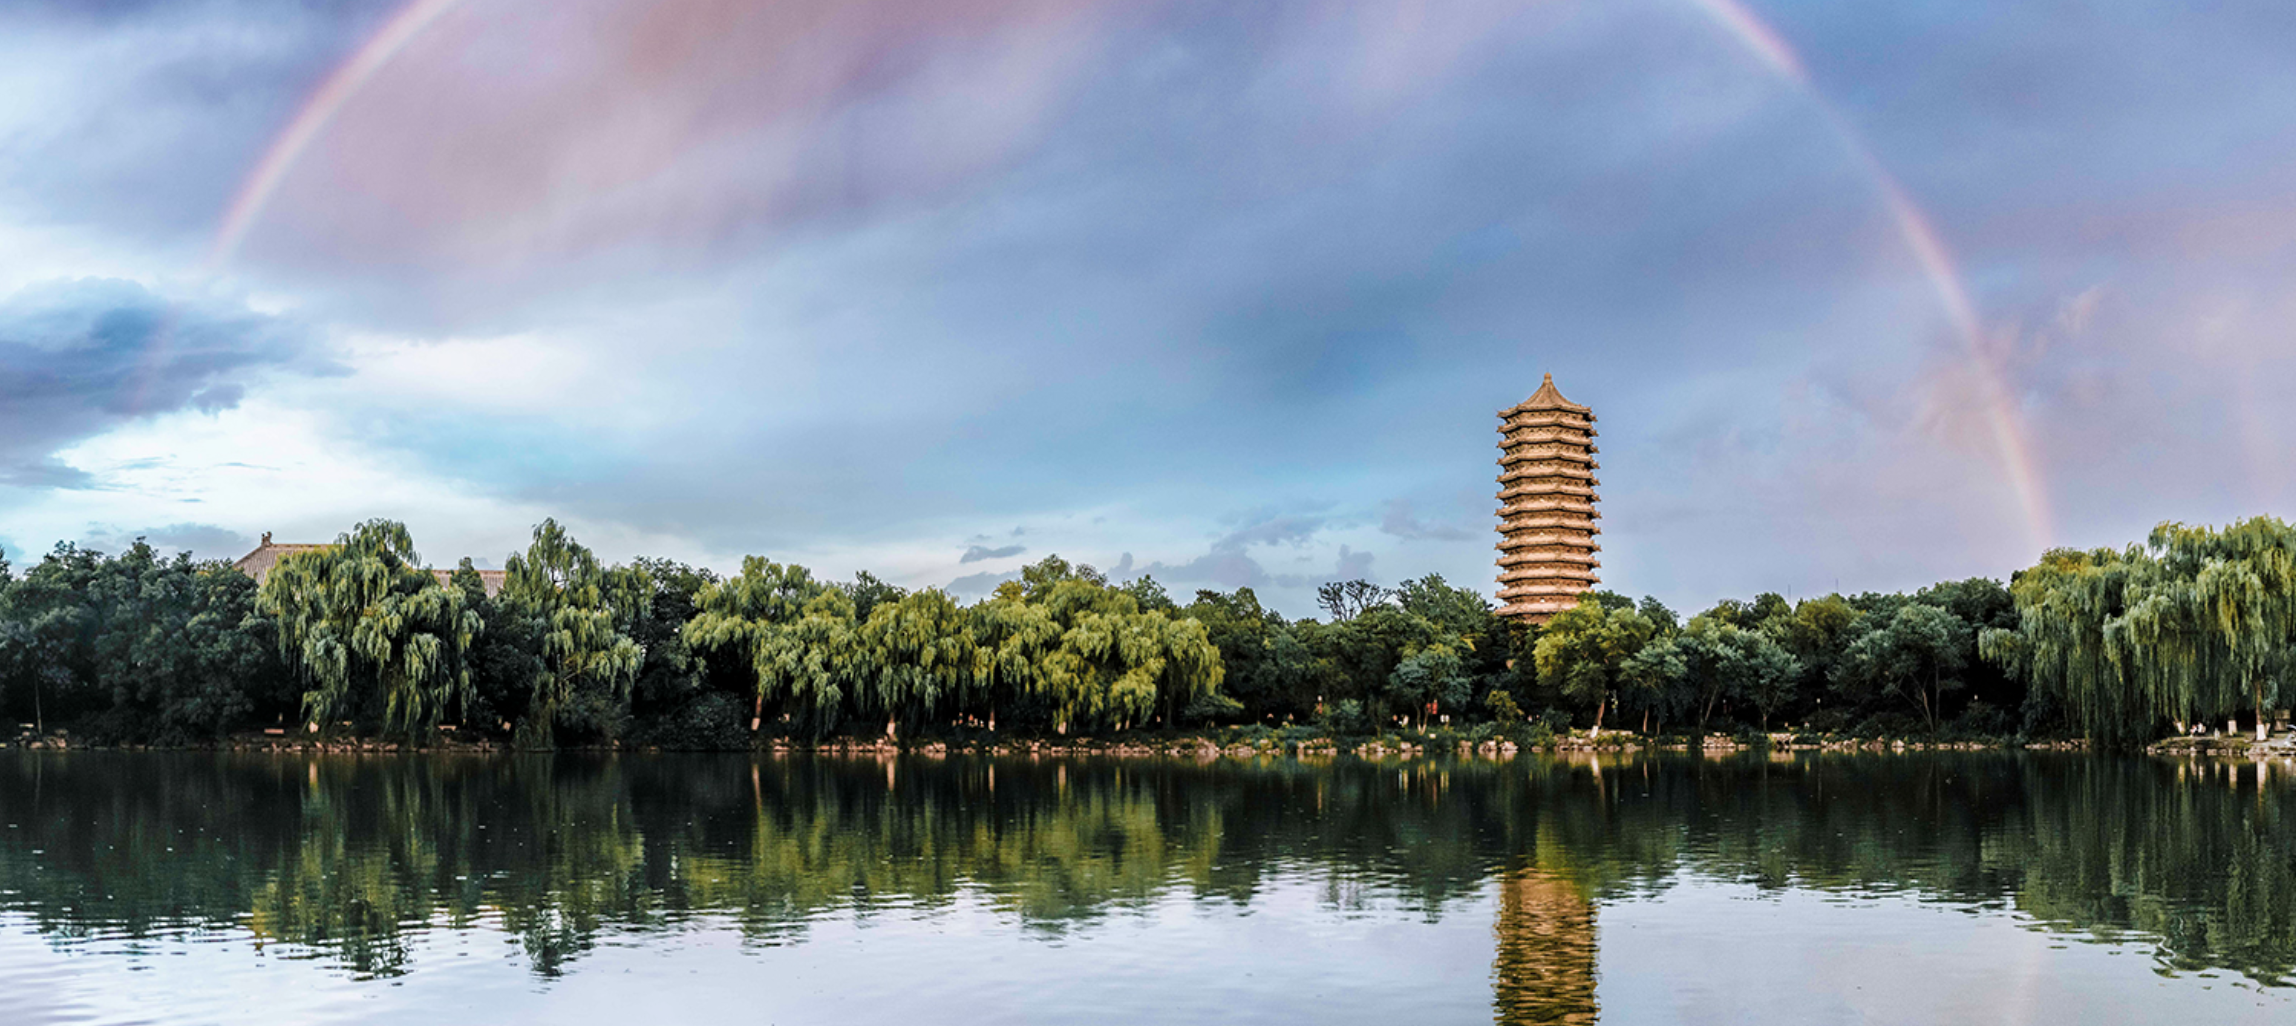
\includegraphics[width=0.9\textwidth]{image/pku.png}
    \caption{Figure Example} 
    \label{fig1}
\end{figure}
\end{lstlisting}

\begin{figure}[!htb]
    \centering
    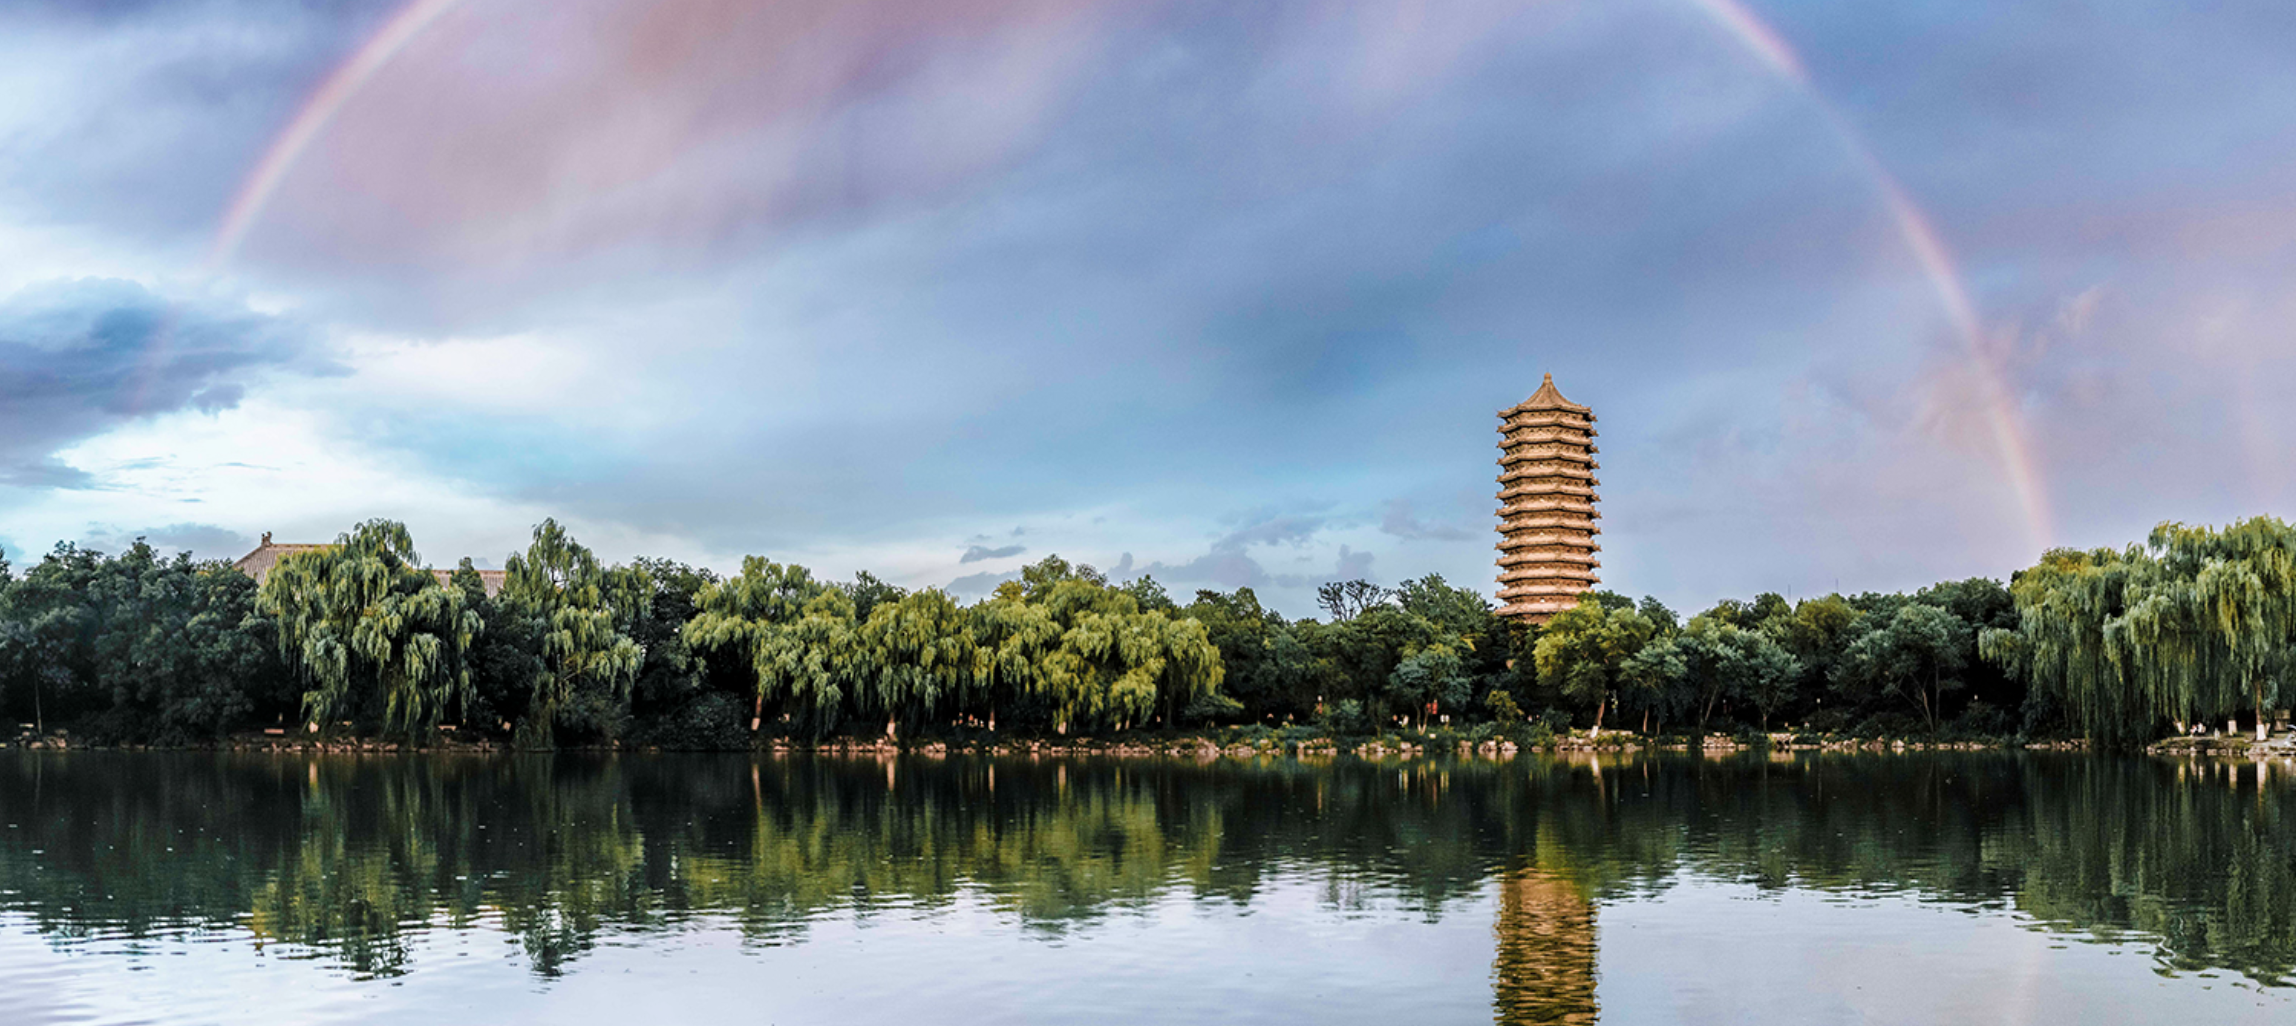
\includegraphics[width=0.9\textwidth]{image/pku.png}
    \caption{Figure Example}
    \label{fig1}
\end{figure}
As shown in \figref{fig1}, this is a picture of Peking University. When referencing images, please use the code: \verb|\figref{fig1}|.

\subsubsection{Tables}
Here is a code example for inserting a table.
\begin{lstlisting}
\begin{table}[!htb]
    \centering
    \caption{Table Example}
    \begin{tabular}{l|c|c|c}
        \toprule
        \textbf{Methods} & \textbf{Metric1}  &  \textbf{Metric2} &  \textbf{Metric3}\\
        \hline 
        Method1~\cite{en1}& XX & XX& XX\\
        \hline
        Method2~\cite{en2}& XX & XX& XX\\
        \hline
        Method3~\cite{en3}& XX & XX& XX\\
        \bottomrule 
    \end{tabular}
    \label{tab1}
\end{table}
\end{lstlisting}

As shown in \tabref{tab1}, this is a statistical table. When referencing tables, please use the code: \verb|\tabref{tab1}|.
\begin{table}[!htb]
    \centering
    \caption{Table Example}
    \begin{tabular}{l|c|c|c}
        \toprule
        \textbf{Methods} & \textbf{Metric1}  &  \textbf{Metric2} &  \textbf{Metric3}\\
        \hline 
        Method1~\cite{en1}& XX & XX& XX\\
        \hline
        Method2~\cite{en2}& XX & XX& XX\\
        \hline
        Method3~\cite{en3}& XX & XX& XX\\
        \bottomrule 
    \end{tabular}
    \label{tab1}
\end{table}


\subsection{Bibliography}

This template uses biblatex to generate the bibliography, the default citestyle and bibliography style are both \lstinline{numeric}. If you want to use biblatex, you must create a file named \lstinline{reference.bib}, add bib items (from Google Scholar, Mendeley, EndNote, and etc.) to \lstinline{reference.bib} file, then cite the bibkey in the \lstinline{tex} file. The biber will automatically generate the bibliography for the reference you cited. Here is a code example for reference: \verb|\cite{key}|.

\subsection{Mathematical Formula}

The use of mathematical formulas is consistent with regular latex documents. This is an example of formula code.
\begin{lstlisting}
\begin{equation}
  L = \int_{R^q} f(x,y) dy
\end{equation}
\end{lstlisting}

The displayed results are as follows:
\begin{equation}
  L = \int_{R^q} f(x,y) dy
\end{equation}


\subsection{Appendix}

The content of the appendix is optional. If there is a need for appendix content, please use the following code to add it; If there is no such requirement, please comment out this section of code.

\begin{lstlisting}
\appendix
\appendixpage
\section{定理1的证明}
\addappheadtotoc
\end{lstlisting}


\printbibliography[heading=bibintoc, title=\ebibname]

\appendix
\appendixpage
\section{Proof of Theorem 1}
\addappheadtotoc


\end{document}
